\chapter{Online Optimization}
This chapter defines, introduces and justifies online optimization  of synchrotron storage rings nonlinear dynamics. A brief overview of optimization algorithms and their classifications is presented. The Robust Conjugate Direction Search (RCDS) algorithm is introduced, as well as the other routines from which it was built upon. This chapter adds no novelty to the literature in optimization. It is an overview for merely pedagogic purposes. It is mostly based on the discussion presented by Numerical Recipes, ref.~\cite{press_numerical_2007}, as well as chapters 7 and 8 of ref.~\cite[]{huang_beam-based_2019} and ref.~\cite{huang_algorithm_2013}.
\section{Defining Online Optimzation}
Consider a system that possesses some sort of figure of merit which depends on the collective state of a set of relevant components, parts, or operation modes which constitute the  parameters or decision variables. There is no mechanistic/deterministic or probabilistic model for the dependence of the figure of merit on the parameters' state, but it is well known that the parameters affect the figure of merit. One may call the relevant parameters knobs, since they can be used to tune the figure of merit.

Now suppose one wants to tune the knobs so the figure of merit reaches a certain value, or so that it is minimized or maximized. This is an optimization problem, with the figure of merit being the objective function. Since the whole system is a black-box, to measure different values for the objective function, i.e., to sample it, the knobs must be varied and the objective fucntion must be measured, a process that may be expensive. The tuning procedure thus consists on trial-and-error repeatition of changing the knobs, evaluating the objection and judging the quality of the changes.

A computer-automated routine or algorithm employing some strategy to seek the desired value or extremum of the objective function while the machine functioning is what we define as online optimization. The program must measure the objective function and read the current state of the knobs, calculate/decide and apply changes to the knobs, measure the objective again, evaluate and judge the quality of the changes over the objective. The process is iterated until the desired outcome is reached.

The Dynamic Aperture (DA) optimization problem suits this heuristic, black-box optimzation schemes very well. The DA is a figure of merit related to the nonlinear dynamics--in SIRIUS' case, the sextupole magnets. There is no analytical/statistical model predicting DA changes given sextupole nudges so the problem cannot be inverted to tune the sextupoles to render the DA a desired value. The tuning procedure must be based on trial-and-error.

\section{Justifying Online Optimization}
\subsection{Why not correct the nonlinear optics?}
Several well-established and effective correction schemes exist for managing linear dynamics in storage rings. These methods rely on measurable figures of merit, enabling diagnostics of linear dynamics and optics. Crucially, they leverage linearly controllable adjustment knobs, allowing for the inversion of the problem—determining how much to tune the knobs to achieve a specific figure of merit. Examples include the widely used Linear Optics from Closed Orbits (LOCO) method, as originally introduced in ref.\cite{safranek_experimental_1997} and routinely applied to SIRIUS \cite{alves_linear_2021, alves_optics_2021}, and other methods utilizing turn-by-turn data evaluation \cite[chapter 5]{huang_beam-based_2019}. These correction schemes ensure that linear optics parameters, dependent on dipoles and quadrupoles, such as optics functions, meet specifications.

Recently, LOCO-inspired schemes have been extended to encompass nonlinear magnets and correct nonlinear optics. These methods have proven successful in addressing the state of sextupoles and octupoles, reportedly enhancing the Dynamic Aperture (DA) and beam lifetime at the MAX-IV, \cite{olsson_nonlinear_2020} and NSLS-II \cite{li_nonlinear_2024} machines. These sophisticated procedures rely on a bottom-up understanding of how off-energy orbits appear for a specific configuration of nonlinear magnets.

Despite the value of these approaches, this master's project adopts the pragmatic, heuristic online optimization strategy. This choice is driven by the immediate need to optimize DA performance for the top-up operation mode and the considerations of available time and task complexity aligning with a master's degree scope. We acknowledge the significance of theory-based correction schemes as crucial next steps for comprehending the machine and establishing connections with the model, a pursuit to be completed in the near future.

\subsection{Are we close enough to the "optimum"?}
Running an online optimization shcheme will find the nearest extremum (minimum/maximum) to the starting point. In other words, if no stochasticity is brought into the routine to diversify the search along the parameter space, it will find local, not global extrema. How can we be sure the local minima are the best solution for the optimization problem? We may not know for sure, but it actually does not matter. A well-performing solution is all we care about as long as other operation parameters are not affected (more details in the next chapter). But there are reasons to believe the local extrema found are actually the global ones, and it has to do with how accelerators are designed and the origins of the deterioration of the dynamic aperture in the machine.

During the design phase of SIRIUS, the strengths and symmetry of the entire nonlinear magnetic lattice were determined through a comprehensive multi-objective optimization process. This process aimed to identify the lattice configuration that would yield the highest dynamic aperture (DA) and optimal lifetime performance based on particle tracking simulations \cite{de_sa_optimization_2016}. The most successful and feasible solution (lattice) resulting from these simulation-based optimization studies was subsequently implemented in the actual machine during the commissioning phase.

The optimization work accounted for the presence of expected errors arising from magnet misalignments or deviations in magnetic fields. These errors introduce additional perturbations that can degrade the dynamic aperture and were intentionally introduced into the model during the simulations for evaluating the figures of merit. Multiple machine models, each with different error configurations distributed across various magnets, were generated. The lattices derived from these models were then evaluated through simulations. The best lattice, determined based on average performance, demonstrated the highest average dynamic aperture and average lifetime in tracking simulations across various error configurations.

In the actual machine, a specific configuration of errors becomes a reality, resulting in a distinct physical magnetic lattice. For this particular lattice, the optimized configuration identified during simulations in the design phase may not necessarily be the one that yields the largest DA or optimal lifetime. However, it is anticipated that optimum sextupole configuration for the realized lattice is not significantly different from the reference configuration chosen and implemented in the machine. Essentially, the assumption is that errors are small and the online optimization procedure, therefore, involves a mere fine-tuning of the strengths of the sextupole lattice to achieve its best-performing configuration, compensating for nonlinear dynamics perturbations and small residual perturbations from linear dynamics. The objective is to tailor the sextupole strengths to match the realized lattice.

\section{Robust Conjugate Direction Search}
Optimization routines and algorithms are commonly categorized based on whether they involve the calculation of derivatives (gradient-based) or rely solely on the comparison of objective function values (gradient-free). The latter can be further classified into direct- or indirect-search methods, depending on whether the extremum search relies on direct comparisons of the objective function or on a mathematical model of it, respectively \cite{press_numerical_2007}.

Both gradient-based and gradient-free strategies rely on the comparison of the objective function at different points of the parameter space. If the objective function suffers from noise this can significantly reduce the efficiency of the optimization routine \cite{press_numerical_2007, huang_beam-based_2019}. In Chap. 7, section 7.3.1 of Ref.~\cite{huang_beam-based_2019}, a review of the most popular optimization algorithms shows how most of them suffer to find minima to, at least, the precision of the noise $\sigma$ the objective function is subjected to.

The Robust Conjugate Direction Search (RCDS) algorithm is an indirect-search, gradient-free optimization algorithm introduced in Ref.~\cite{huang_algorithm_2013}. The algorithm comprises a main loop for constructing and managing optimal search directions along the knobs space (Powell's Method) and a one-dimensional optimizer responsible for a noise-aware search for the minimum along a given direction. Demonstrated in \cite{huang_algorithm_2013} and \cite[section 7.3.3]{huang_beam-based_2019}, the algorithm can optimize the objective function with a precision at least equivalent to the objective-function noise, making it suitable for online optimization problems. Specifically, for accelerator controls and optimization, the algorithm has been successfully applied to optimize beam steering and optics matching during injection \cite{huang_algorithm_2013}, reduce horizontal emittance \cite{huang_algorithm_2013, huang_online_2015}, and optimize dynamic aperture \cite{huang_algorithm_2013, huang_online_2015,liuzzo_rcds_2016,olsson_online_2018,yang_online_2022} at machines such as SPEAR3, NSLS-II, MAX-IV, and ESRF. It has become the standard tool for optimizing the DA.

To this date, the only 4th-generation machine RCDS has been applied to was MAX-IV. The machine has five sextupole families and five octupole families. When used as knobs subject to relevant operation constraints, such as chromaticity, the resulting parameter search space was 6-dimensional \cite{olsson_online_2018}. SIRIUS, on the other hand, has 21-sextupole families. The application of RCDS in a 4GSR with such a large search space, as seen in SIRIUS, is of great interest to the community, especially for upcoming upgrades and new 4GSR projects currently under construction.

\subsection{One-dimensional search optimizers}
RCDS distinct noise robustness is due to the cumulative effect of minor modifications of well-known indirect-search routines. To grasp how it works, a brief overview on its predecessors is presented next.

% Suppose we are searching for the optimal configuration of a system with a single knob, such as minimizing a certain figure of merit. Manually, we could slowly adjust the knob and measure the objective, scanning for the minimum. This process involves scanning along the possible values of the tuning knob, turning it up or down as long as the objective improves, and stopping when it starts to deteriorate. For knobs existing along the real number line, this is essentially a line scan. How can we teach a computer to perform the same task?

Let $f(x)\in\mathbb{R}$ be the objective function depending on the single knob $x\in\mathbb{R}$. The goal of optimizing $f$ is accomplished through a direct search over its domain. Since maximizing a function is equivalent to minimizing the same function multiplied by $-1$, in the following discussion, we shall refer to minimization only. The search for the minimum is usually preceded by initially \textit{bracketing} the minimum. We seek points $a < b < c$ in the domain such that $f(b)$ is smaller than both $f(a)$ and $f(c)$. If $f$ is reasonably smooth, we can be certain there will be a minimum in the interval $(a, c)$. Standard bracket routines for well-behaved, noiseless objective functions can be found in the literature \cite[section 10.1]{press_numerical_2007}. They mostly consist on starting from an initial point, scanning the line "downhill" until $f$ stops decreasing. This allows identifying a first guess for the minimum, $x=b$, as well as $x=a$ and $x=c$, the borders of the interval containing it: the brackets. The bracketing procedure can be seen as a coarse-grained scan performed initially.

After bracketing, the minimum is then more finely searched by a rountine referred to as line search or line scan. The most common line search methods are the \textit{golden section search} and \textit{parabolic interpolation} \cite[sections 10.2 and 10.3]{press_numerical_2007}. Parabolic Interpolation involves fitting a parabola to the values $f(a), f(b), f(c)$. Moving along the parabola minimum leads to the estimate for $f$'s minimum in a single leap.
% \begin{itemize}
%     \item Golden Section Search: This method progressively scans $f$ within the brackets, updating the brackets at each iteration in such a manner it shrinks at each round. Eventually, the bracket spans only a small interval, specified by the user. The machine precision $\epsilon$ is often indicated. The guess for the minimum is taken as the mid-point along the interval with a precision of $\epsilon/2$.
%     \item
% \end{itemize}
Both of these methods rely on comparisons of the objective function at different points in the parameter space. They assume that the objective function $f$ is deterministic and they trust their observed behavior. In other words, they are completely unaware of any experimental noise in the system. In what follows, we assume what we actually measure in the control-room is $f(x) + \xi$, where $\xi\sim\mathcal{N}(\mu=0, \sigma)$ is a random variable modeling the experimental noise, with $\sigma$ being expected noise error, $\sigma^2 = \text{Var}[\xi]$.

For the optimization of noisy objective functions, the line optimizer introduced in Ref.~\cite{huang_algorithm_2013} incorporates minor modifications to traditional bracketing and the parabolic interpolation line scan rotutine. Unlike traditional bracketing, RCDS enforces the stricter condition that $f(b) + 3\sigma < f(a)$ and $f(b) + 3\sigma < f(c)$, where $\sigma$ is the standard deviation of the objective function values, its experimental noise. In other words, RCDS brackets are obtained by scanning downhill no only until the function stops decreasing, but until it increases again by at least three times the expected errors. This increases the likelihood that the observed trend represents real behavior of the objective function rather than noise. Figure~\ref{fig:bracketing} illustrates RCDS bracketing routine. Starting from $x_0$, $f(x_1)$ is sampled. Since it is no grater than $f(x_0)+3\sigma$, the scan continues up to $x_2$, which is updated as the best guess for the minimum. The process is repeated and the minimum is then updated to $x_3$. When sampling $f(x_4)$, condition $f(x_4) > f(x_3) + 3\sigma$ is true and the bracketing stops. The brackets consists on the interval $(x_0, x_4)$ and the best guess for the minimum is $x_3$.

Next, for the line search, a parabola is fitted within the brackets using the points previously sampled. The parabola vertex is taken as the objective function minimum. Prior to fitting, however, an outlier verification routine scans the measured values for $f$. If any point is identified as an outlier, it is discarded, and the fitting process is repeated without it, if we are still left with a suficient number of sampled values of $f$. If that is not the case, additional measurements are carried out.

\begin{figure}
    \begin{minipage}{0.48\textwidth}
        \centering
        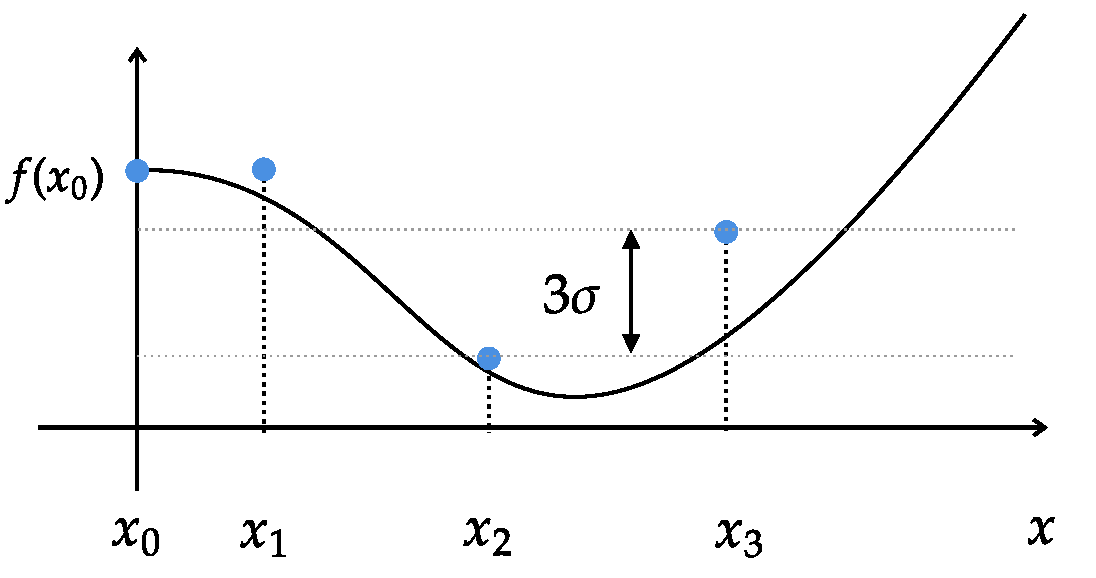
\includegraphics[width=\textwidth]{Images/bracketing.pdf}
        \caption{Illustration of RCDS bracketing: scan the objective function $f$ downhill, updating the guess for the minimum, until $f$ stops decreasing and increases by more than $3\sigma$ compared to best guess for the minimum.}
        \label{fig:bracketing}
    \end{minipage}
    \hfill
    \begin{minipage}{0.48\textwidth}
        \centering
        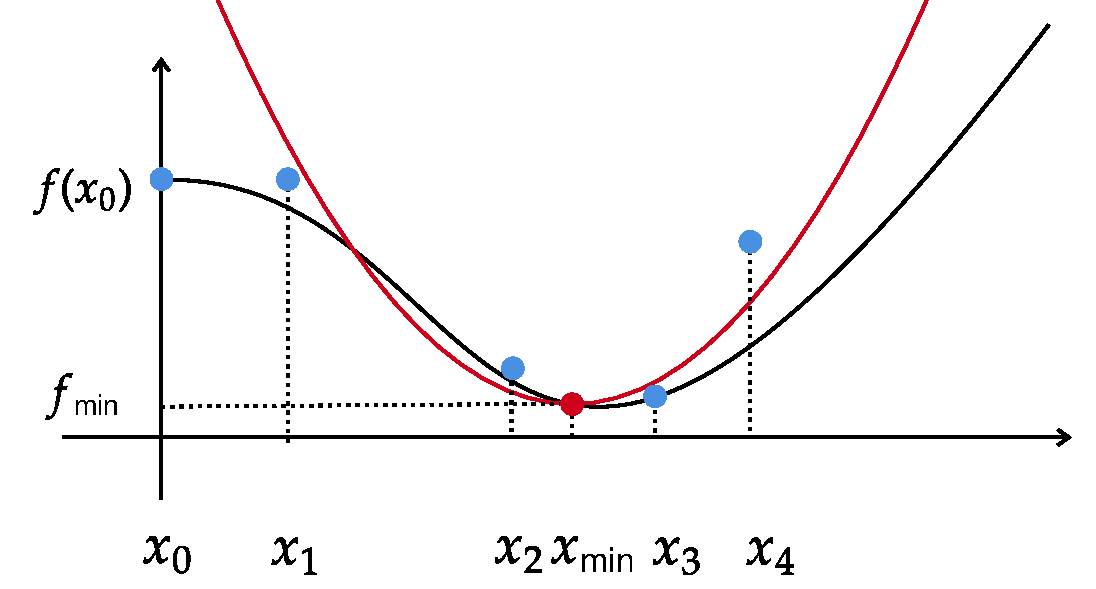
\includegraphics[width=\textwidth]{Images/linescan.pdf}
        \caption{Illustration of RCDS line-scan procedure: parabolic fitting over a curated set of points within the brackets (with outliers removed). The parabola vertice is the best guess for $f$'s minimum.}
    \end{minipage}
\end{figure}
\todo[inline]{FIX FIGURES: uneven scanning steps along the domain. Steps actually increase progressively, up to $0.1$.}
\subsection{Powell's conjugate directions}
% Next we investigate how to optimize a several-variables objective function. We note that a multi-dimensional problem can be reduced to a line-search if we choose to focus on a single direction.
How could we optimize an objective function $f(\vb{x})\in\mathbb{R}$ depending on the set of $p$ parameters $\{x_i\}_{i=1,\dots,p}$? The simplest idea is to iteratively optimize nudging each knob individually: optimize $f$ by changing $x_1$, while the other knobs remain fixed. Next, optimize by changing $x_2$ only, and so forth. In other words, each one of the knobs defines a direction whose basis vector is $\vu{e}_i$, correspoinding to a unit change of the knob. This is easy to automate with the noise-robust line-optimzer introduced in the previous section.

Formally, we are reducing a multi-dimensional optimzation problem into a series of line-searches. That is, given an intial configuration of the parameters (an initial position) $\vb{x}_0$, and a direction $\vu{n}$, we have the one-dimensional problem to minimize $g(\delta)=f(\vb{x}_0 + \delta \vu{n})$. The minimum is  then $f(\vb{x}_0 + \delta_* \vu{n})$, where $\delta_* = \text{arg min}_\delta g(\delta)$. In the previous paragraph, we specialized to $\vb{n}=\vu{e}_i$, and iterated for $i=1,\dots, p$.

\begin{figure}[htb]
    \centering
    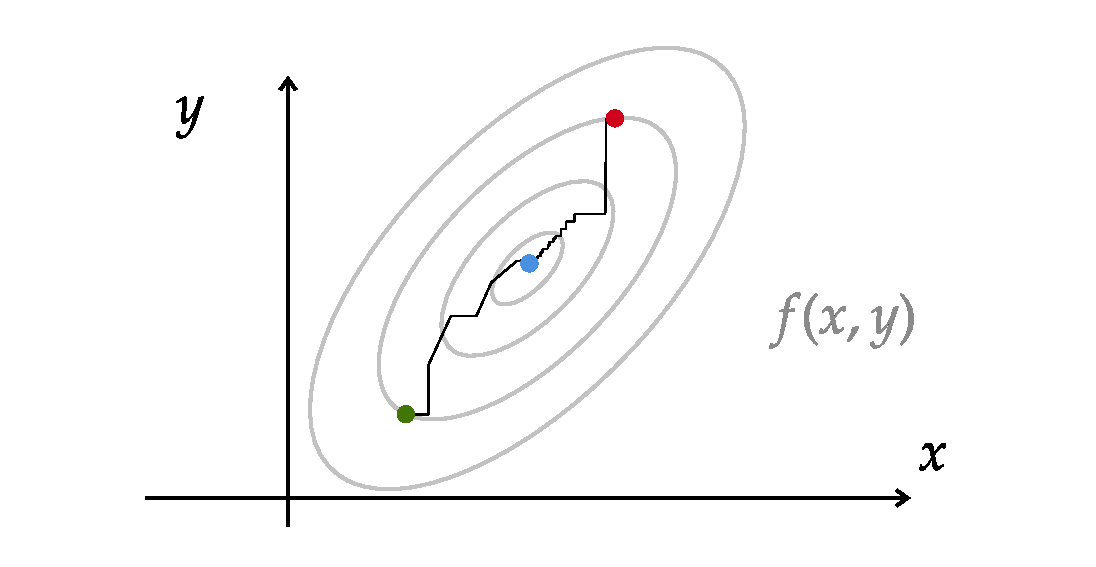
\includegraphics[width=0.9\textwidth]{Images/powell_loop.pdf}
    \caption{Comparison of iterated line-searches until $f(x,y)$'s minimum along canonical unit vectors (path from red dot to blue dot) and along vectors chosen according to Powell's procedure of conjugate directions (path from green to blue dot).}
\end{figure}

As can be seen in figure, scanning along each orthogonal directioon can be time-consuming, specially for some functions with long narrow valleys at some angle with the coordinates basis vectors. This strategy thus is suboptimial when evaluation of the objective function is expensive.

The reason why using unit basis vectors can be so inneficient is because optimizing along a given basis vector spoils down minimization carried out in the any other of them. So the processes needs to be iterated. A more efficient strategy consists on constructing a set of special non-interfering direction vectors for which the minimizationsare preserved when optimizing in a different driection.
% Going back to the one-dimensional problem of minimizing along a direction $\vb{u}$, $\delta_* = \text{arg min}\ g(\delta) = f(\vb{x}_{0}+\delta\vu{u})$, we know that, at the minimum, we must have vanishing derivative: $g^{\prime}(\delta_*)=\grad f(\vb{x}_{0}+ \delta_* \vu{u})\cdot \vu{u}=0$. Therefore, the gradient is perpendicular to $\vu{u}$ at $\delta_*$.

% Consider now the quadratic-form approximation for the objective function around point $\vb{x}_0$, taken as the origin.
% \begin{equation}
%     f(\vb{x})=f(\vb{x}_0)+\grad f(\vb{x}_0)\cdot \vb{x} + \frac{1}{2}\vb{x}\cdot\vb{H}(\vb{x}_0)\cdot\vb{x},
% \end{equation}
% where, as usual, $(\grad f(\vb{x}_0))_i = \pdv*{f(\vb{x}_0)}{x_i}$ is the gradient, and $(\vb{H})_{ij} = \pdv*{f(\vb{x}_0)}{x_i}{x_j}$ is the Hessian matrix. Up to such approximation, differentiation of the previous expression reaveals the gradient can be approximated by
% \begin{equation}
%     \grad f(\vb{x}) = \grad f(\vb{x}_0) + \vb{H}(\vb{x}_0)\cdot \vb{x}
% \end{equation}
% and thus is changed by
% $$\delta(\grad f ) = \vb{H}(\vb{x}_0)\cdot \delta \vb{x}$$
% upon a step $\vb{\delta \vb{x}}$. Suppose we have optimzed along direction $\vb{u}$, so $\grad f(\vb{u}) = \grad f(\vb{x}_0) + \vb{H}\cdot \vb{u}$. Now, optimizing along $\vb{v}$ will be non-interfering if the gradient stays orthogonal to $\vb{v}$, that its
The necessary condition for direction vectors $\vb{u}$ and $\vb{v}$ to be non-interfering is (proof in the apendix)
\begin{equation}
    \vb{v}\cdot\vb{H}\cdot\vb{u}=0,
\end{equation}
where $(\vb{H})_{ij} = \pdv*{f(\vb{x}_0)}{x_i}{x_j}$ is the Hessian matrix for function $f$. The $\vb{u}$ and $\vb{v}$ directions are said to be conjugate directions.

The problem now consists on finding an appropriate set of $p$ conjugate directions, so we can optimize $f(\vb{x})$ along them. Let $\{\vb{u}_i\}$ denote our directions set. Powell proved conjugate directions can be constructed as follows
\begin{enumerate}
    \item Set the initial directions as the basis vectors: $\vu{u}_i=\vu{e}_i, i=1,\dots, p$.
    \item Save the starting point (initial parameters state) as $\vb{x}_0$;
    \item For $i=1,\dots, p$ minimize along $\vu{u}_i$. Save the minimimum as $\vb{x}_i$.
    \item For $i=1,\dots p-1$ set $\vu{u}_i\leftarrow\vu{u}_{i+1}$
    \item Set $\vb{u}_p=\vb{x}_p - \vb{x}_0$. Normalize to obtain $\vu{u}_p$.
    \item Minimize along $\vu{u}_p$. Name the found minimum as the new $\vb{x}_0$ and repeat the procedure until reaching a certain number of evaluations or until some stopping condition is reached.
\end{enumerate}

That is, from steps 1--3. we optimize along each one of the unit basis vectors, updating the minimum. When finishing optimization along ${x}_p$, the current minimum will be $\vb{x}_p$. In step 4 we discard the first direction, rename directions $\vb{u}_{i+1}$ to $\vb{u}_i$, and set as our new $p$th direction the vector from the starting point $\vb{x}_0$ to the the current minimum.

Powell proved that repeating this procedure $k$ times for a quadratic form produces a set of directions whose last $k$ vectors are mutually, pairwise conjugate, in the sense of the Hessian matrix. So $p$ iterations exactly minmizes the quadratic form. The method is also quadratically convergent: each iteration doubles the number of significant figures of the candidate minimum for the quadratic form.

There is a problem in throwing away  for $\vu{u}_1$ for $\vb{x}_p - \vb{x}_0$ every iteration: at some point the lines start to fold up on each other and lose linear independence. As a result the function can end up minimized only within a subspace of parameter space. To fix this, you can reinitialize the directions to the basis vectors after an iteration along the $p$ directions, or use any new set of orthogonal directions.

The somewhat counterintuitive solution suggested by Powell is to discard not necessarily $\vu{u}_1$ in favor of the new direction, but the direction along which $f$ had its largest decrease so far. This is justified because this direction is likely have a largest component along the new proposed conjugate direction. Accepting this advice results in a set of $p$ directions which are no longer mutually conjugate by the end of $p$ iterations. As a result, the method will no longer be quadratically convergent

Powell also posits some conditions in which is best not to add any new directions, keeping the old set from the previous iteration. These are presented in the appendix, as well as the pseudo-code for the Powell loop.

In summary, Powell's direction set loop calculates and manages directions adaptatively, deciding when to change old directions in favor of newly calculated conjugated vectors, and when to avoid the changes to control build-up of linear depencence

In practice, using conjugate directions accounts to finding a good set of directions in which the number of steps along the vectors is reduced. They provide ``shortcuts'' towards the minimum in the objective landscape.

RCDS implementation by the authors of ref.\cite{huang_algorithm_2013} is available in Matlab and Python in their \href{https://github.com/SPEAR3-ML/RCDS}{GitHub repository}. Several other implementations from other accelerator teams can also be found. The code used in this dissertation was implemented in Python and is available in the "optimization" directory of the \href{https://github.com/lnls-fac/apsuite}{Accelerator Physics Suite (apsuite)} repository \cite{apsuite}. The pseudo-code for the bracketing, linescan and outlier verification routines as well as Powell's conjugate directions loop is available in appendices. (TODO)
